% Manuscript skeleton — representation_collapse project.
% Canonical question/claims: doc/auto/research-charter.md.
% Every number in this manuscript must trace to a doc/auto/ artifact or the
% independent scientific review; see paper/README.md for the placeholder policy.
\documentclass[11pt]{article}

\usepackage[T1]{fontenc}
\usepackage[utf8]{inputenc}
\usepackage{lmodern}
\usepackage[margin=1in]{geometry}
\usepackage{amsmath,amsthm,amssymb}
\usepackage{booktabs}
\usepackage{graphicx}
\usepackage{xcolor}
\usepackage{soul}
\usepackage{enumitem}
\usepackage[round,authoryear]{natbib}
\usepackage[colorlinks=true,linkcolor=blue!50!black,citecolor=blue!50!black,urlcolor=blue!50!black]{hyperref}
\usepackage{xurl}   % allow \url/\path to break anywhere (long artifact paths)
\usepackage[capitalise,noabbrev]{cleveref}

% Unicode characters that may appear in the snapshot bibliography.
\DeclareUnicodeCharacter{2212}{-}
\DeclareUnicodeCharacter{2009}{\,}
\DeclareUnicodeCharacter{00A0}{~}

% Theorem environments.
% Propositions carry their own counter so that Proposition k is Pk in the text.
\theoremstyle{plain}
\newtheorem{proposition}{Proposition}
\newtheorem{lemma}{Lemma}
\newtheorem{corollary}{Corollary}
\theoremstyle{definition}
\newtheorem{definition}{Definition}
\newtheorem{assumption}{Assumption}
\theoremstyle{remark}
\newtheorem{remark}{Remark}

% Placeholder and evidence-status macros.
% \todo{...}      highlighted placeholder; plain text only (no \cite, no math).
% \evidence{...}  inline evidence-status tag. Allowed values:
%   analytic | infrastructure | executed-verified | executed-unreduced |
%   inconclusive | attributed-unverified | protocol | planned | conditional
\definecolor{todoback}{RGB}{255,240,140}
\definecolor{evidencecolor}{RGB}{0,90,150}
\sethlcolor{todoback}
\newcommand{\todo}[1]{\hl{TODO: #1}}
\newcommand{\evidence}[1]{{\small\textcolor{evidencecolor}{[\textsc{evidence: #1}]}}}

% Math shorthands.
\newcommand{\R}{\mathbb{R}}
\newcommand{\E}{\mathbb{E}}
\newcommand{\tr}{\operatorname{tr}}
\newcommand{\rank}{\operatorname{rank}}
\newcommand{\diag}{\operatorname{diag}}
\newcommand{\Cov}{\operatorname{Cov}}
\newcommand{\PR}{\operatorname{PR}}
\newcommand{\norm}[1]{\lVert #1 \rVert}
\newcommand{\DID}{\mathrm{DID}}
% \hash{hex}: typewriter hash that may break after any character.
\ExplSyntaxOn
\NewDocumentCommand{\hash}{m}{\texttt{\small\rc_hash_break:n{#1}}}
\cs_new_protected:Npn \rc_hash_break:n #1
  { \tl_map_inline:nn {#1} { ##1 \allowbreak } }
\ExplSyntaxOff

\title{When does repetition erase what a recurrent network needs?\\[0.4em]
\large Useful-history loss under controlled periodic forcing in fixed-weight recurrent models}
\author{Mehrab Hamidi\thanks{\todo{affiliation and contact}} \and \todo{coauthors, order and affiliations}}
\date{Manuscript skeleton, 2026-10-12. Internal draft; not for distribution.}

\begin{document}
\maketitle

% Scope: analytic controls and a verified native-competence audit.
\begin{abstract}
Does repetition erase information from recurrent state, or merely change how that information is represented and read out? Low covariance dimension, contracting tangent dynamics, and poor task performance do not resolve this question individually. We formulate an experiment in which a fixed-weight network writes a cue once, processes either a periodic distractor body or an equal-length matched control, and then answers a query. We organize analytic nulls and counterexamples that constrain its interpretation. For fixed affine dynamics, cue differences are independent of body order at equal horizon; commuting switched-affine dynamics obey an analogous null under matched symbol counts. Nevertheless, order-dependent offsets can change native error without erasing the cue. Conversely, locally contracting dynamics can preserve categorical memories in distinct basins, while isotropic attenuation can reduce noise-resolved memory without changing normalized dimension. These controls motivate separate measurements of conditioned geometry, complete-state propagation, and task information. An audit of four single-seed GRU/LSTM pilots illustrates the prerequisite: all fail short-horizon native competence, making repetition-induced forgetting inconclusive. The contribution is a falsification framework and a controlled experimental design for recurrent-memory claims; the current evidence does not establish a learned collapse mechanism.
\end{abstract}

\section{Introduction}
\label{sec:introduction}

Repeated computation can concentrate representations into a small subspace. This observation appears in graph oversmoothing \citep{oono2020exponential,roth2024rank}, attention rank loss \citep{pure_attention_rank}, and dimensional collapse in representation learning \citep{jing2022dimensional}. Its significance depends on what the representation must preserve. A compact state may encode every required variable; a high-dimensional state may consist largely of irrelevant fluctuations. In recurrent models, a further ambiguity arises: local contraction can coexist with useful memory when different cues select different stable responses \citep{pals2024-phase-locked-memory}. A geometric observation alone cannot distinguish efficient compression from destructive forgetting.

We consider a concrete question: after a recurrent model has acquired task-required information, does a periodic distractor body cause more loss than a matched non-periodic body of the same length? The network's weights, written values, query, and number of updates remain fixed across the comparison. The intervention changes motif ordering while matching symbol counts, bigram counts, run lengths, endpoints, and the final motif. This isolates a specified ordering contrast, rather than a universal effect of ``periodicity'': higher-order input statistics necessarily remain different.

Answering the question requires distinguishing three objects. A covariance spectrum describes the geometry of a selected ensemble. A tangent product describes propagation of infinitesimal state perturbations along a particular trajectory. Native behavior and controlled decoding describe different forms of access to task information. Their relationships require assumptions. Isotropic attenuation preserves normalized covariance dimension while reducing signal relative to fixed noise. Nuisance compression lowers dimension while preserving the target. Separate stable basins retain categorical labels despite contracting local spectra. An arm-dependent readout offset changes error even when the cue-dependent state component is identical. \Cref{fig:controls} makes these distinctions concrete.

We contribute a compact set of analytic controls, a matched-body measurement design, and an empirical audit that demonstrates why verified native competence must precede a harmful-retention claim. The controls assemble established dynamical and information-theoretic ideas into explicit falsifiers: fixed affine and commuting switched-affine systems cannot support particular ordering explanations; local stability does not determine global cue retention; and normalized dimension does not determine noise-resolved information. We use \emph{diagnostic non-identifiability} in this limited sense: a diagnostic value need not determine whether the required information survives. The individual ingredients are not claimed as new dynamical theorems.

The audit covers four trained model/task combinations: GRU and LSTM, each with categorical and continuous targets. Every selected checkpoint fails short-horizon competence. Consequently, their later errors cannot establish erasure of successfully acquired information. This negative outcome is useful as a methodological case study, but it supplies neither a periodicity effect nor evidence of general recurrent collapse. The paper therefore centers the inference problem and its controls, with the remaining empirical question stated explicitly.

\section{Related work}
\label{sec:related}

\paragraph{Driven dynamics and memory.}
Echo-state theory separates loss of initial-condition dependence from dependence on input history \citep{jaeger2001,manjunath2013}. Input-driven Lyapunov analysis characterizes local perturbation growth \citep{vogt2020}, while input repetitions can alter the number of attracting responses \citep{ashwin2023-echo-repetitions}. Most directly, \citet{pals2024-phase-locked-memory} demonstrate cue-selected, stable phase-locked memories and analyze their Floquet stability. This work already establishes that periodic forcing and local contraction can preserve categorical information. Continuous attractors provide a complementary mechanism for analog memory \citep{seung1996}. Our comparison requires both preservation and loss as admissible outcomes.

\paragraph{Geometry and usable information.}
Fisher memory quantifies retained information relative to specified noise and distinguishes normal from nonnormal recurrence \citep{ganguli2008-memory-traces}. Covariance spectra \citep{hu2022} and entropy effective rank \citep{roy2007effective} measure different objects. Sampling and task complexity further constrain observed dimension \citep{gao2017dimensionality}. These antecedents motivate reporting absolute variance and conditioned cue recovery alongside normalized dimension; the latter is not an information bound. Likewise, probe control tasks and relevance tests distinguish decodability from native task use \citep{hewitt2019-control-probes,ravichander2021-probe-relevance}.

\paragraph{Graph and repeated computation.}
Graph oversmoothing, rank collapse, and the Jacobian connection between graph and recurrent networks are established \citep{oono2020exponential,roth2024rank,arroyo2025bridging}. T-GRAB supplies temporal-graph periodic-memory tasks and GC-LSTM evaluations \citep{dizaji2025tgrab}; these motivate the broader setting but provide no reproduced graph result here. Input reinjection in equilibrium models \citep{deep_equilibrium} also differs from once-written streaming memory because the model retains access to the input. Relative to these literatures, our contribution is the explicit combination of equal-horizon motif matching, complete-state conditioning, analytic ordering nulls, and a competence prerequisite. We make no priority claim for Floquet analysis, dimension measurement, or attractor memory.

% Canonical source: doc/auto/research-program.md (exact discrete dynamics, Floquet applicability,
% dimension contract); doc/auto/periodicity-analysis-v1.md (closure contract); charter §4.
\section{Setting: complete state, discrete dynamics and estimands}
\label{sec:setting}

\subsection{Notation and complete state}
A recurrent model with fixed parameters $\theta$ has complete persistent state $s_t\in\R^n$ and update
\begin{equation}
  s_{t+1} = F_\theta(s_t, x_t),\qquad
  J_t = \partial_s F_\theta(s_t, x_t)\in\R^{n\times n},\qquad
  P_{t,L} = J_{t+L-1}\cdots J_{t+1}J_t .
  \label{eq:update}
\end{equation}
Derivatives are taken at fixed external inputs and parameters. The complete state includes every quantity carried across time: for a GRU of width $H$, $s_t=h_t\in\R^{H}$; for an LSTM, $s_t=[h_t,c_t]\in\R^{2H}$; for a one-layer node-wise graph LSTM on $N$ nodes, $s_t\in\R^{2NH}$ together with the node ordering and flattening manifest, because graph convolution couples nodes and a per-node block is not the transition Jacobian. Persistent buffers, convolution histories, matrix memories and caches, where present, are part of $s_t$ or are declared fixed. We record whether inputs are teacher-forced or generated in closed loop; in a closed loop, derivatives through generated inputs belong in $J_t$.

An episode is a WRITE prefix, a body and a terminal QUERY. The WRITE prefix carries a cue $u\in\mathcal U$ (required coordinates) and nuisance values $v$; the body $h=(x_0,\dots,x_{H-1})$ carries no memory values; the query reveals the selector $q$ only at the final step. Write $s_H(u,v,h)$ for the complete state immediately before the query. Two bodies $h,h'$ are \emph{matched} when they have equal length and the matching statistics of \cref{sec:design}. The periodic arm repeats one motif $R$ times; the horizon is $R$.

\subsection{Discrete framework; no continuous embedding}
All analysis is of the discrete map \eqref{eq:update}. Writing $F(s,x)-s$ as a vector field defines an Euler surrogate at step one; the exact flow of that ODE is not in general $F$, and no continuous-time embedding is needed for a period-map analysis. The inherited draft's conversion to a continuous-time limit (\cref{app:inherited}) is therefore not used.

\subsection{When Floquet terminology applies}
\begin{definition}[Verified periodic orbit]
\label{def:verified-orbit}
Fix a period $T$. The input is $T$-periodic on the analysed window if $x_{t+T}=x_t$ realized vector by vector. The complete-state trajectory is closed at tolerance $(\varepsilon_{\mathrm{abs}},\varepsilon_{\mathrm{rel}})$ if, after a declared burn-in, consecutive phase-matched blocks of $T{+}1$ states satisfy $\norm{s_{t+T:t+2T}-s_{t:t+T}}\le\varepsilon_{\mathrm{abs}}$ and the same difference is at most $\varepsilon_{\mathrm{rel}}$ times the larger block norm (floored at $10^{-12}$). The orbit period is the observed one, which may be a multiple of the input period.
\end{definition}
For an exactly closed orbit, $J_{t+T}=J_t$ follows from \eqref{eq:update}, and
\begin{equation}
  M_t = J_{t+T-1}\cdots J_t
\end{equation}
is the one-period tangent map whose eigenvalues $\mu_i$ are discrete Floquet multipliers. Under approximate closure, Jacobian periodicity is a separate numerical check with its own residual; the v1 periodicity protocol reports it but does not certify it, so every product there retains the finite-time label. The following statements are direct for these maps: $|\mu|<1$ denotes per-cycle modal contraction at the verified orbit, not monotone contraction within the cycle (P8); $|\mu|=1$ alone does not prove an oscillatory clock, since defective unit-modulus blocks grow polynomially and a multiplier $+1$ need not oscillate; a forced discrete orbit has no automatic neutral phase multiplier; repeating an input does not make the Jacobian constant, because the state can differ between repeats; and a one-step rotation at frequency $m/T$ raised to the power $T$ has one-period multiplier $1$, so a block pattern such as AABB does not predict fourth-root-of-unity multipliers of its one-period map. Under an input-specific echo-state condition the driven response has a period dividing the input period \citep{manjunath2013}; without such a condition a longer period, several coexisting responses, or no periodic response are admissible outcomes.

\subsection{Finite-time propagators}
When closure is not verified, or inputs are fresh stochastic draws, we report for any window the singular values $\sigma_i(P_{t,L})$, the largest gain $\norm{P_{t,L}}_2$, and finite-time rates $\ell_i(t,L)=\log\sigma_i(P_{t,L})/L$ in units of inverse update. These are conditional on the realized forcing; input-perturbation sensitivity is a different measurement. Eigenvalue modulus and singular value answer different questions: a nonnormal product can have spectral radius below one and finite-window gain above one. Long products are formed by JVP/VJP with scaled QR or SVD and are checked against dense products and central finite differences on small cases; zero singular values are reported as rank deficiency at the stated precision, never replaced by a floor. A leading partial spectrum supports only a partial claim.

\subsection{Three estimands}
\paragraph{Covariance geometry.}
For a cue-conditioned cloud $\{s_H(u_j,v,h)\}_{j=1}^{N_{\mathrm{cue}}}$ at fixed $v$, $h$, phase and horizon, let $C$ be the centered sample covariance with eigenvalues $\lambda_i\ge0$ and $p_i=\lambda_i/\sum_k\lambda_k$. We report the participation ratio $\PR(C)=(\sum_i\lambda_i)^2/\sum_i\lambda_i^2$, the covariance entropy dimension $D_{\mathrm{ent}}=\exp(-\sum_i p_i\log p_i)$, the smallest ranks $D_{90},D_{95}$ explaining 90\% and 95\% of variance, the absolute variance $\tr C$, the spectrum, the numerical rank at declared tolerance, the sample count and the centering and normalization used. For LSTM we report $h$, $c$ and $[h,c]$; for graphs, node-wise, whole-graph and pooled representations separately. Normalized dimension is undefined for an all-zero cloud. Sampling ceilings apply: time-only covariance of an exact period-$P$ orbit has rank at most $P-1$, and a cloud of $N_{\mathrm{cue}}$ cues has rank at most $N_{\mathrm{cue}}-1$ (P6). Pooling body histories measures driver diversity and is rejected by the implementation as a conditioned measurement.

\paragraph{Tangent propagation.}
Finite-time propagators and, where \cref{def:verified-orbit} holds, Floquet multipliers, as above; with absolute amplification alongside any normalized tangent dimension.

\paragraph{Behavior and information.}
Native task error (categorical accuracy; continuous normalized MSE defined as $\mathrm{MSE}/(1/3)$ against the fixed population variance of $\mathrm{Uniform}[-1,1]$); held-out ridge probes fit on training cues with train-only standardization and shuffled-label controls; counterfactual cue separation $\norm{s_H(u,v,h)-s_H(u',v,h)}$ as a finite difference rather than a derivative; and causal interventions: complete-state swaps between matched histories, same-phase transplants, and direction-specific corruption and rescue against equal-energy random and nuisance shams. Probe success is not native use; probe failure is not information absence; a full-state transplant establishes causal relevance of state, not mediation by a dimension change.

% Scope: elementary diagnostic results, not a new general theory of forgetting.
% Repository derivations: doc/auto/theory-propositions.md; inherited drafts remain unchanged.
\section{What collapse diagnostics can identify}
\label{sec:theory}

An ordering intervention changes the sequence of state transitions. Whether it
changes memory depends on the cue-bearing channel, the decoder, and the noise
model. The following elementary results separate these dependencies. They
organize established linear-memory and attractor arguments
\citep{ganguli2008-memory-traces,seung1996,pals2024-phase-locked-memory}; no
novelty is claimed for the individual results. Proofs and additional
counterexamples appear in \cref{app:proofs}.

\subsection{Ordering nulls concern the cue channel}

Let $E(u)\in\R^n$ be the state after writing cue $u$, and let
$h=(x_0,\ldots,x_{H-1})$ be a distractor body independent of $u$.
All comparisons use the same encoder and body length $H$.

\begin{proposition}[Affine cue-channel ordering nulls]
\label{prop:affine}\label{prop:commuting}
For $s_{t+1}=As_t+c_{x_t}$ with $s_0=E(u)$,
\begin{equation}
 s_H(u,h)=A^H E(u)+k_h,\qquad
 k_h=\sum_{j=0}^{H-1}A^{H-1-j}c_{x_j}.
 \label{eq:affine-channel}
\end{equation}
Consequently cue differences, cue derivatives (when defined), and the
body-conditioned cue covariance are body-independent; the covariance is
$A^H\Cov(E(u))(A^H)^\top$.
More generally, for $s_{t+1}=A_{x_t}s_t+c_{x_t}$, if the symbol matrices
commute pairwise, equal symbol counts imply the same cue propagator
$\Phi_h=A_{x_{H-1}}\cdots A_{x_0}$ and the same centered cue covariance.
These are noiseless statements, also valid conditional on shared fixed noise.
\end{proposition}

The null concerns centered, body-conditioned cue information. It does not imply
equal native task error. Nor does commutativity eliminate noise effects:
intermediate noise is propagated through suffix products, which can differ
between equal-count bodies. With fixed $A$, cue-independent additive noise
with the same \emph{joint} law across arms produces the same terminal-noise law;
matching its one-step marginals alone is insufficient.

\begin{corollary}[Readout offsets can change error without changing memory]
\label{cor:offset}
Suppose two terminal states differ by a cue-independent translation and,
if noisy, have matched translated joint laws with the cue. A body-informed
decoder can compensate that translation and attain equal optimal risk.
For a fixed affine native head, let $e$ be its control-arm residual and
$\Delta$ its deterministic output shift. The squared-loss gap is
\begin{equation}
 \E\norm{e+\Delta}^2-\E\norm{e}^2
 =2\E[e]^\top\Delta+\norm{\Delta}^2.
 \label{eq:offset-gap}
\end{equation}
\end{corollary}

Thus an error contrast can identify readout sensitivity while leaving cue
recoverability unchanged. Conversely, noncommuting transitions permit, but do
not guarantee, unequal cue products or unequal recovery risk. The standard
adjacent-swap bound in \cref{lem:swaps} quantifies a possible product change;
it neither assigns a harmful direction to periodic order nor bounds decoder
error without further assumptions.

\subsection{Dimension, contraction, and recovery are distinct}

Consider $u\sim\mathcal N(0,I_d)$, stored as $s_H=a^Hu$ with $0<a<1$.
At every finite horizon, the signal covariance has participation ratio $d$,
although its trace is $d a^{2H}$. If the measured state is
$y_H=s_H+\varepsilon$ with independent
$\varepsilon\sim\mathcal N(0,\sigma^2I_d)$ and $\sigma>0$, its covariance
also has participation ratio $d$, while the optimal squared recovery risk is
\begin{equation}
 \E\norm{u-\E[u\mid y_H]}^2
 =\frac{d\sigma^2}{a^{2H}+\sigma^2}\longrightarrow d.
 \label{eq:attenuation-risk}
\end{equation}
Without that noise, $a^{-H}s_H$ recovers $u$ exactly. A scale-invariant
dimension statistic therefore cannot identify reliable memory loss; a noise
or precision model is essential. The converse is also possible:
$s_H=(u,a^Hv)$ for independent isotropic $u\in\R^d,v\in\R^k$ retains $u$
exactly while participation ratio decreases from $d+k$ toward $d$.

Local contraction is likewise compatible with finite categorical memory.
This is the elementary counterpart of phase-locked memory in driven recurrent
networks \citep{pals2024-phase-locked-memory}.
\begin{proposition}[Contracting categorical memory]
\label{prop:basins}
Let $\phi_t=0.2(-1)^t$, $r_t=s_t-\phi_t$, and
$s_{t+1}=g(r_t)+\phi_{t+1}$ with $g(r)=1.5r-0.5r^3$.
The two period-two responses $s_t=\pm1+\phi_t$ have zero tangent multipliers.
The tubes $|r_t\mp1|\le0.05$ are invariant and contracting, yet
$\operatorname{sign}(s_t)$ recovers their binary label for every $t$.
\end{proposition}

Contraction within a basin does not measure separation between basins. Exact
smooth memory of a continuum has a different local requirement, familiar from
continuous-attractor models \citep{seung1996}.
\begin{proposition}[Exact smooth memory requires neutral directions]
\label{prop:continuous}
Let $U\subset\R^d$ be open and let $E:U\to\R^n$ and
$\mathcal D:\R^n\to\R^d$ be $C^1$, with $\mathcal D(E(u))=u$.
Then $\rank DE(u)=d$. If a $C^1$ period map $\mathcal P$ also satisfies
$\mathcal P(E(u))=E(u)$ on $U$, then
$D\mathcal P(E(u))DE(u)=DE(u)$: its tangent map has at least $d$
independent eigenvectors with eigenvalue one.
\end{proposition}

This is an exact preserved-family statement. Finite-sample mean-squared
competence alone supplies neither a local singular-value bound nor a neutral
multiplier. Finally, a forced periodic response can persist with strictly
contracting multipliers (\cref{prop:scalar}), and stable eigenvalues allow
transient gain (\cref{prop:nonnormal}). Periodic activity, covariance dimension,
and tangent stability each require a separate task-memory measurement.

\section{A matched-order memory experiment}
\label{sec:design}

\paragraph{Task and pairing.}
Each episode contains sixteen WRITE observations, a distractor body, and a terminal QUERY (\cref{fig:design}). Eight written coordinates are task-relevant and eight are nuisance. Values are either equiprobable among sixteen categorical levels or independent $\mathrm{Uniform}[-1,1]$ draws. The query selects one required coordinate; neither it nor the body carries the answer. An eight-register oracle is an explicit sufficient-memory control. Paired arms share required values, nuisance values, query, and total updates.

The body uses twelve-symbol motifs over $\{\mathrm A,\mathrm B,\mathrm X\}$, each containing three As, three Bs, and six Xs. The five motifs share bigram counts, unit run lengths, and the prefix \texttt{AX} and suffix \texttt{BX}; the full library is in \cref{app:protocol}. One arm repeats a selected motif $R$ times. The control draws motif identities, fixes its final motif to the same selected motif, and rejects whole-body proper periods. Local repeated substrings remain allowed. At $R=1$, the arms coincide. With unit dwell, the body length is $H=12R$. Matching does not equalize all higher-order correlations or predictability, so the treatment is precisely this motif-ordering intervention.

\paragraph{Acquisition before retention.}
The proposed diagnostic ladder distinguishes a single WRITE followed immediately by its query, all sixteen WRITEs with no body ($R=0$), and short bodies ($R=1,2$). Even $R=0$ requires early values to survive subsequent WRITEs. The stronger design requires every queried coordinate to reach at least $95\%$ categorical accuracy or normalized MSE at most $0.05$ at all three latter horizons in both arms. Normalized MSE divides raw MSE by $1/3$, the continuous population variance. These are proposed criteria: the executed pilots used weaker aggregate gates of $25\%$ accuracy or raw MSE $0.25$ at $R=1,2$, and failed them. Checkpoint selection uses validation task loss, independently of geometric measurements and arm-effect signs.

\paragraph{Behavioral estimands.}
For native error $E_a(R)$, define
\begin{equation}
 \delta_R=E_{\mathrm{per}}(R)-E_{\mathrm{ctl}}(R),\qquad
 \DID=\delta_{16}-\delta_2 .
 \label{eq:contrasts}
\end{equation}
The within-training-support horizons $R=2,16$ compare excess error and its change with retention length. A positive $\DID$ can occur with both arm differences negative; it does not alone establish harm. Independent training seeds are the replication units. Confirmation requires seed-paired uncertainty, a prespecified effect-size threshold and comparison family, and a fixed treatment of competence failures. Ten fresh seeds and a $0.02$ smallest effect are candidate design values, not a completed preregistration. One seed per cell supports no training-population confidence interval. Longer horizons are extrapolation and require separate interpretation.

\paragraph{Localizing a failure.}
Matched episodes are evaluated after WRITE, before QUERY, and after QUERY. Cue-conditioned complete-state clouds separate acquisition, body propagation, and query/readout effects. Train-fit probes use held-out cues, shuffled-label controls, and recorded standardization floors. Offset-compensated decoding tests the alternative in \cref{cor:offset}. State swaps and direction-specific perturbations or rescues test task use against random and nuisance shams; a complete-state swap alone cannot establish mediation by dimension. Restoring an earlier state also changes the operating point, so a rescue requires matched disruption controls. Finite cue differences and robustness to declared noise complement local tangent products. Native precision, coordinate ULP spacing, and fixed-weight FP64 replay are reported separately; replay changes numerical arithmetic and does not retroactively repair stored states.

\paragraph{Decision rule.}
The design permits preserved memory, equal forgetting in both arms, readout failure, and inconclusive outcomes. A learned erasure claim requires prior competence, excess error at a specified horizon, diminished recoverability under the declared measurement model, and evidence that the implicated state change affects behavior beyond shams. A dimension correlation alone does not meet that standard.

\section{Analytic controls and a competence audit}
\label{sec:results}

\subsection{Constructed controls separate the diagnostics}
\Cref{fig:controls} makes four distinctions concrete. Isotropic attenuation
reduces cue variance without changing participation ratio. Two forced attracting
basins retain a categorical label despite zero derivative on their reference
cycles. An affine system has identical centered cue clouds under different
forcing orders while its fixed native readout incurs different offset errors.
Finally, a noncommuting switched-linear system permits an ordering effect in
optimal linear recovery under common terminal noise; its sign changes with the
noise level. These are explicit constructions, not observations of trained
networks or a claim that periodic ordering generally harms memory.
The figure generator passes all 36 mechanism-calibration checks and verifies
the risk formula separately through the singular values of the channel.

\begin{figure}[t]
\centering
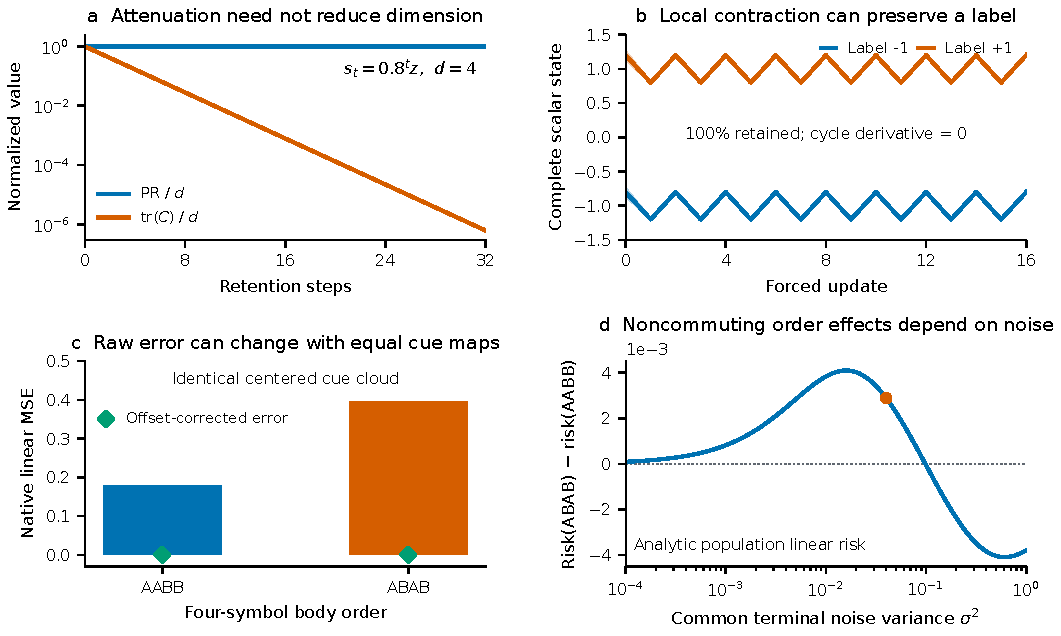
\includegraphics[width=\linewidth]{figures/analytic_controls.pdf}
\caption{\textbf{Diagnostic dissociations in constructed systems.}
(a) $s_t=0.8^t z$, with isotropic four-dimensional cues: normalized variance
decays while normalized PR remains one.
(b) Two phase-forced cubic attractors retain their labels; shaded envelopes
vary the initial perturbation by at most 0.05 and are not confidence intervals.
(c) Different affine offsets change native error while the cue map is unchanged;
offset correction removes the error.
(d) For two noncommuting matrices and matched symbol counts, the population
linear-risk difference between ABAB and AABB changes sign as common terminal
noise varies. The orange point uses noise covariance $0.04I$. These short
analytic bodies do not satisfy the full motif-matching design.}
\label{fig:controls}
\end{figure}

\subsection{The trained pilots fail the prerequisite for harmful-loss inference}
Four GRU/LSTM categorical/continuous pilots completed 1,500 optimization steps,
with one training seed (0) per cell and validation-selected checkpoints.
Saved predictions, complete-state arrays and compact reductions were independently
verified. Each behavior estimate uses 256 paired held-out episodes per horizon;
these episodes do not replace independent training seeds.
\Cref{fig:pilot-audit} shows the decisive outcome: all four cells fail even the
original engineering criterion at $R=1,2$, before the stricter research criterion.
Both categorical models achieve 5.47\%, 6.25\% and 5.08\% accuracy at
$R=1,2,16$ in both arms, against 6.25\% chance.
Continuous MSE is 0.998--1.018 times the exact saved-target zero-predictor MSE.
Periodic-minus-control MSE contrasts are at most $1.20\times10^{-7}$ in
magnitude. These near-zero contrasts cannot establish equivalence of competent
memory mechanisms.

\begin{figure}[t]
\centering
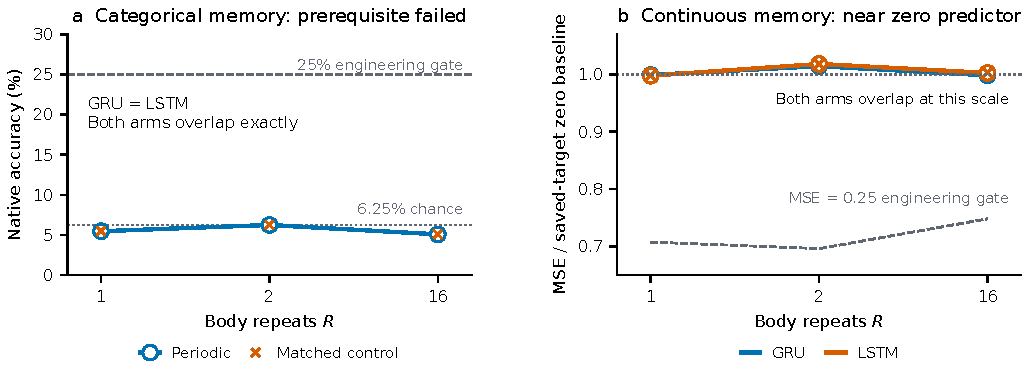
\includegraphics[width=\linewidth]{figures/pilot_audit.pdf}
\caption{\textbf{Native competence is absent in the verified seed-0 pilots.}
(a) The categorical GRU and LSTM have identical aggregate accuracies;
periodic circles and control crosses coincide exactly.
(b) Continuous errors are normalized by the zero-predictor error on the same
targets. Color denotes architecture; circles/crosses denote periodic/control
arms, which overlap at this display scale. Dashed lines show the original
25\% accuracy and 0.25 MSE engineering gates. No training-seed uncertainty
is estimated from a single fit per cell.}
\label{fig:pilot-audit}
\label{fig:pilots}
\end{figure}

\paragraph{Residual decodability qualifies the failure.}
At $R=2$, every cue-conditioned cloud has a held-out real-label probe advantage
over its shuffled-label control. Categorical probe accuracy spans
20.95--22.75\% for GRU and 14.75--15.53\% for LSTM; these ranges describe
four fixed-driver/arm clouds per cell, not uncertainty intervals.
Thus poor native behavior does not imply that all cue information is absent.
The $R=16$ probe advantages are inconsistent, but interpreting this difference
requires care: feature standardization uses a $10^{-8}$ floor, and the observed
state variations approach float32 coordinate spacing.
\Cref{app:probe-scale} gives an exact invertible-encoding counterexample in which
that floor alone makes ridge error approach the zero-predictor baseline.
It diagnoses a possible measurement confound without attributing the pilot
contrast to that confound. Full cloud measurements appear in
\cref{app:pilot-details}.

\paragraph{What the evidence licenses.}
The pilots establish failed native competence under this training protocol.
They do not localize the failure to acquisition, retention or readout, and
neither support nor falsify harmful periodic memory loss in competent models.
Independent checkpoint-only reduction verifies attenuation in both arms, with
precision-sensitive nonzero cue separation. Twenty subsequent local fits fail
full-coordinate competence before any distractor body, despite partial successes.
Twelve separate singleton-query fits pass at addresses 7 and 15 and fail at
address 0 (\cref{app:acquisition}); those different weights do not establish
joint eight-address recall. Acquisition, native readout and the causes of the
address-dependent pattern remain unresolved.

\section{Discussion and conclusion}
\label{sec:discussion}

The central inference problem is asymmetric. A successful decoder demonstrates surviving information within its evaluation regime; a failed decoder cannot exclude every alternative code. A counterexample disproves a universal implication from contraction or low dimension to forgetting; it does not establish how often a trained model uses that counterexample. Our analytic controls exploit this asymmetry to delimit permissible explanations.

The affine null is especially useful: equal-horizon cue propagation is unchanged by body order, although offsets can alter native error. In nonlinear networks, input-dependent gating, changing operating points, and basin transitions remove this restriction, but observing such ingredients does not identify which causes a failure. Finite cue separation, task-sensitive propagation, and controlled interventions are needed together. Likewise, lower dimension with preserved performance is compatible with sufficient compression; contracting local spectra with separated cue basins are compatible with categorical memory.

The pilots in \cref{fig:pilots} expose an earlier failure of inference. Failed native competence makes later poor performance an ambiguous retention measurement; it does not localize failure to acquisition rather than query/readout. The resulting contribution is a falsification framework supported by analytic constructions and an empirical audit. Whether matched repetition erases acquired information in competent trained models remains an open empirical question.

\section{Limitations}
\label{sec:limitations}

The analytic results concern stated affine, local, or exact-memory assumptions; they do not predict a generic GRU or LSTM outcome. Their individual foundations are established, and the paper's contribution is their use as a coherent diagnostic contract.

The cue-memory audit has one training seed in each of four synthetic model/task cells, and none passes competence. It cannot estimate effects across training runs or establish repetition-induced forgetting. Probe regularization at tiny state scales also confounds comparisons across horizons. Float64 analysis of saved float32 states cannot restore lost numerical information.

The ordering intervention matches selected statistics, not every temporal dependency. Its final-motif exposure difference is structural (\cref{app:motif-exposure}); even a supported ordering effect would require further interventions to attribute it to one periodicity mechanism. Covariance dimension depends on conditioning, sample size, and coordinate metric; local tangent dynamics do not characterize global basin structure. State interventions can themselves cause off-manifold disruption. These limitations require explicit controls rather than a single collapse score.

The graph appendix covers one capped corrected GC-LSTM on one graph realization, with compact-output verification rather than independent binary-state reanalysis. It does not reproduce the complete original multi-model, five-seed figure or establish causal retention loss. No native cross-modal transfer is demonstrated; rendering one latent task in several modalities would not by itself establish such transfer. The proposed stronger competence and statistical design remains separate from the executed pilot evidence.

\section{Reproducibility and evidence provenance}
\label{sec:reproducibility}

\paragraph{Frozen training evidence.}
The four pilots ran source \hash{9004a0c114a8b7c5335dca3d5247449fd10b5ffa}, with \path{configs/experiments/initial-phase-v1.json} and \path{configs/experiments/vector-pilot-v1.json}. The recorded runtime was Python 3.11.13, PyTorch 2.6.0 with CUDA 12.4, and NumPy 2.4.6; GRU runs used A100 devices and LSTM runs H100 MIG slices. Source, checkpoint and output checks were independently reconciled in \path{doc/auto/initial-phase-results.json}, which also records scheduler identifiers. Training seed, checkpoint selection, evaluation units and all cloud measurements appear in Appendices~B--C. The qualifications are in \path{doc/auto/initial-phase-scientific-review.md}.

\paragraph{Reproducing figures and manuscript.}
Plotting uses the committed evidence JSON and deterministic calculations. The \texttt{paper} and \texttt{experiments} dependency groups are locked in \texttt{uv.lock}. From the repository root:
\par\noindent
\begin{minipage}{\linewidth}
\small
\begin{verbatim}
uv sync --locked --all-groups
PYTHONPATH=src .venv/bin/python code/analysis/make_paper_figures.py
.venv/bin/python code/analysis/summarize_prefix_acquisition.py
cd paper
latexmk -pdf -interaction=nonstopmode -halt-on-error \
    -outdir=build main.tex
\end{verbatim}
\end{minipage}
\par

The figure manifests record input/output hashes, versions, parameters and plotted values. At source \hash{999d88d8679c0f353c6bb7fb4f5ab8433a7e730c}, the local suite passes 239 tests with zero skips, including the original 14 constructor/oracle tests and additive complete-state, inference and worker-lifecycle checks; measurement and mechanism calibrations check ten and thirty-six conditions, respectively. Analytical fixtures validate measurements and identities, not a trained-model mechanism.

\paragraph{New corrected graph evidence.}
The appendix fit uses source \hash{6d89c657c41cf38ff3dd074a1e886b4bd2b26c4c}
(Mila job 11321105); selected evaluation and retained-state analysis use
\hash{1891bdd59bf47b944c8799ae345ebb26b9a4e497}
(jobs 11322413 and 11322422). The accepted evaluation-result digest is
\hash{8acc39f47225e53f0b5b208c32460505687340dcf1ab1aaae646b1860c9d0091};
the compact state-analysis digest is
\hash{1722d1b2165a704124bdb05305dfb654e7702a7aa24a5da459551a9723920f38}.
Figure manifests under \path{doc/auto/figures/figure10-gclstm-pilot-2026-10-19/}
bind the accepted inputs and copied PDFs. The frozen behavioral and trajectory
protocols are \path{doc/auto/figure10-within-motif-descriptive-2026-10-19.md}
and \path{doc/auto/figure10-trajectory-diagnostics-2026-10-19.md}.
Actual offline W\&B histories and result metadata artifacts are verified;
remote delivery is not. Compact verification checks reported state arithmetic,
not an independent reanalysis of the retained binary trajectory. This evidence
must not be conflated with the excluded inherited graph assets.

\paragraph{Evidence excluded from the reported results.}
A checkpoint-only periodicity batch ran source \hash{458bc9cfce474b8e11e433e33bf132faf5032387}. Independent reduction at source \hash{ec1c489fc97c2e6cf94fd58e8a4e04dd3e8ba901} checks 64 finite-time tangent windows and 1,536 step Jacobians, with descriptive native FP32/FP64 cue and closure comparisons recorded in \path{doc/auto/periodicity-independent-results.json}. Two cue histories cannot estimate representation dimension, tolerance-qualified closure does not certify an exact orbit, and all original competence gates fail. These arrays establish no empirical Floquet or causal-memory result. Inherited graph figures still lack recovered checkpoint and trajectory provenance and are excluded; the separately executed corrected reconstruction in \cref{app:graph-reconstruction} has its own new evidence chain. Causal interventions and competent multi-seed replications remain prospective.


\bibliographystyle{plainnat}
\bibliography{references}

\appendix
% Self-contained derivations for the diagnostic statements in the main text.
\section{Proofs and supporting counterexamples}
\label{app:proofs}

\subsection{Cue-channel ordering and readout effects}

\paragraph{Proof of \cref{prop:affine}.}
Unrolling the switched-affine recurrence gives
\begin{equation}
 s_H=\Phi_hE(u)+k_h,\qquad
 \Phi_h=A_{x_{H-1}}\cdots A_{x_0},\qquad
 k_h=\sum_{j=0}^{H-1}
       (A_{x_{H-1}}\cdots A_{x_{j+1}})c_{x_j},
 \label{eq:unrolled-switched}
\end{equation}
where an empty product is the identity. Subtraction cancels $k_h$,
differentiation gives $D_us_H=\Phi_hDE(u)$, and covariance is invariant to
translation. Fixed $A$ yields $\Phi_h=A^H$. Pairwise commutativity yields
$\Phi_h=\prod_\sigma A_\sigma^{n_\sigma}$, so equal counts give equal products.
All covariance claims require a common cue law with finite second moments.
For fixed $A$ and cue-independent additive noise,
$s_H=A^HE(u)+k_h+\sum_jA^{H-1-j}\eta_j$. A common joint noise law gives the
same propagated law; if the noise is independent of the cue, its covariance
adds to the displayed signal covariance. With independently drawn episode
noise, individual cue differences also contain noise differences. With
switched matrices, even independent identically distributed process noise can
produce unequal terminal covariance: two scalar transitions $a,b$, with
independent variance-$\tau^2$ noise after each update, give terminal-noise
variances $(1+b^2)\tau^2$ in order $ab$ and $(1+a^2)\tau^2$ in order $ba$,
although both cue products equal $ab$. \qed

\paragraph{Proof of \cref{cor:offset}.}
Subtracting $k_h$ makes the joint law of state and target identical between
bodies. Composing any decoder with this translation gives the same risk under
any fixed loss; the affine-decoder class is also closed under translations
when it includes an intercept. This is an equality of attainable optimal
risks, not of finite-sample fitted probes. Expanding
$\norm{e+\Delta}^2-\norm{e}^2$ proves \cref{eq:offset-gap}.
If bodies vary across paired samples, the general expression is
$2\E[e^\top\Delta]+\E\norm{\Delta}^2$; the factorization in the main text
requires a deterministic shift. The required compensation is body-specific:
a single intercept per arm need not suffice for a mixture of bodies. \qed

\begin{remark}[Noncommutativity is insufficient]
\label{prop:noncommuting}
If equal-count products differ, at least one matrix pair fails to commute,
by the contrapositive of \cref{prop:affine}. The converse is false.
Take $A=\diag(1,-1)$ and
$B=\left(\begin{smallmatrix}0&1\\1&0\end{smallmatrix}\right)$.
Then $AB=-BA$, but $(AB)^2=(BA)^2=-I$.
Moreover, the unequal products $AB$ and $BA$ are orthogonal, so their cue
channels have identical optimal recovery risk with independent isotropic Gaussian terminal noise
and unrestricted decoding: rotating the observation converts either into the
same channel $u+\varepsilon$. Thus a changed product is itself insufficient
for a changed recovery risk.
\end{remark}

\begin{lemma}[Adjacent-swap bound]
\label{lem:swaps}
Let two words of length $H\ge2$ have the same symbol counts and be connected
by $K$ adjacent swaps. If $\norm{A_\sigma}_2\le L$ with $L>0$ and
$\kappa=\max_{\sigma,\tau}\norm{A_\sigma A_\tau-A_\tau A_\sigma}_2$, then
\[
 \norm{\Phi_h-\Phi_{h'}}_2\le K L^{H-2}\kappa.
\]
\end{lemma}
\begin{proof}
For a single swap, factor the difference into a common left product, the
commutator, and a common right product. The common products contain $H-2$
factors in total, so submultiplicativity bounds the difference by
$L^{H-2}\kappa$. Sum the $K$ differences along the swap sequence and use the
triangle inequality. Equal-count words admit such a sequence by successive
adjacent transpositions. The corresponding change in a cue difference is at
most $KL^{H-2}\kappa\norm{E(u)-E(v)}$. This standard telescoping bound omits
affine offsets and process-noise propagation, and has no lower bound or sign.
\end{proof}

\subsection{Covariance geometry and noisy recovery}

\begin{proposition}[Sampling ceilings and coordinate dependence]
\label{prop:ceilings}\label{prop:pr}
A centered cloud of $N$ states in $\R^n$ has covariance rank at most
$\min(N-1,n)$. A time-only sample of an exactly $P$-periodic orbit has rank at
most $\min(P-1,n)$. For nonzero covariance $C\succeq0$,
$\PR(C)=(\tr C)^2/\tr(C^2)$ is invariant to positive scalar multiplication
and orthogonal coordinate changes, but not to anisotropic invertible scaling.
Writing $p_i=\lambda_i/\tr C$ on the positive eigenvalues,
\[
 1\le\PR(C)=e^{H_2(p)}\le e^{H_1(p)}\le\rank C.
\]
The upper three quantities coincide exactly for equal positive eigenvalues;
equality also with one requires rank one. For zero covariance, normalized
dimension is undefined.
\end{proposition}
\begin{proof}
Centered sample rows sum to zero. An orbit sample additionally lies in the
affine span of at most $P$ points. These give the rank bounds. Scaling and
orthogonal invariance follow directly from traces. In contrast,
$C=I_2$ transformed by $\diag(1,\epsilon)$ has
$\PR=(1+\epsilon^2)^2/(1+\epsilon^4)\to1$ as $\epsilon\downarrow0$,
although the transformation is invertible for every $\epsilon>0$.
Finally, $\PR=1/\sum_i p_i^2$. Jensen's inequality gives
$-\sum_i p_i\log p_i\ge-\log\sum_i p_i^2$, and the entropy maximum on a
support of size $r$ is $\log r$, attained exactly at the uniform law.
\end{proof}

\begin{lemma}[Linear recovery channel]
\label{prop:channel}
For independent zero-mean $u,\varepsilon$ with covariances
$\Lambda\succ0,\Sigma\succ0$, the best linear estimator of $u$ from
$y=Gu+\varepsilon$ has squared error
$\tr[(\Lambda^{-1}+G^\top\Sigma^{-1}G)^{-1}]$.
For Gaussian $u,\varepsilon$, this is also the unrestricted Bayes risk.
\end{lemma}
\begin{proof}
The best linear estimator is
$\Lambda G^\top(G\Lambda G^\top+\Sigma)^{-1}y$.
Its error covariance is
$\Lambda-\Lambda G^\top(G\Lambda G^\top+\Sigma)^{-1}G\Lambda$;
the Woodbury identity yields the displayed expression. Gaussian conditioning
makes the same estimator the conditional mean. Setting
$G=a^HI_d$, $\Lambda=I_d$, and $\Sigma=\sigma^2I_d$ gives
\cref{eq:attenuation-risk}. For non-Gaussian cues, a nonlinear decoder can
improve on the linear risk.
\end{proof}

For the complementary nuisance-compression example in the main text, put
$q=a^{2H}$. The covariance of $(u,a^Hv)$ is
$\diag(I_d,qI_k)$ and its participation ratio is
$(d+kq)^2/(d+kq^2)$. Its derivative with respect to $q\in(0,1)$ is
$2dk(d+kq)(1-q)/(d+kq^2)^2>0$ for $d,k>0$, so participation ratio decreases
with $H$ while the readout selecting $u$ remains exact.

\subsection{Categorical basins and continuous memory}

\paragraph{Proof of \cref{prop:basins}.}
The shifted coordinate satisfies $r_{t+1}=g(r_t)$, with
$g(\pm1)=\pm1$ and $g'(\pm1)=0$. At $r=1+\delta$,
$g(r)-1=-1.5\delta^2-0.5\delta^3$; odd symmetry gives the same magnitude
bound at $-1$. For $|\delta|\le0.05$, the next error is at most
$0.0038125<0.05$, proving invariance, and
$|g'(r)|\le1.5(2\cdot0.05+0.05^2)=0.15375<1$, proving contraction.
At each phase the two tubes are separated by at least $1.9$;
$|\phi_t|=0.2$ ensures that their signs also agree with their labels.
The period-two tangent product along either reference response is zero.
This proves retention for all times within the stated tubes, not global
attraction to those tubes. \qed

\paragraph{Proof of \cref{prop:continuous}.}
Differentiating $\mathcal D(E(u))=u$ yields
$D\mathcal D(E(u))DE(u)=I_d$, so $DE(u)$ has rank $d$.
Differentiating $\mathcal P(E(u))=E(u)$ yields
$D\mathcal P(E(u))DE(u)=DE(u)$. Each of the $d$ independent columns of
$DE(u)$ is therefore a unit-eigenvalue eigenvector. Both identities must hold
on an open set. A small average reconstruction error cannot replace them:
in one dimension, $E_\epsilon(u)=u+\epsilon\sin(u/\epsilon)$ and
$\mathcal D(s)=s$ have pointwise squared error at most $\epsilon^2$,
yet $E_\epsilon'$ vanishes wherever $\cos(u/\epsilon)=-1$.
Approximate competence alone therefore gives no positive local gain bound. \qed

\subsection{Periodic response, transient gain, and reinjection}

\begin{remark}[A forced oscillation needs no neutral multiplier]
\label{prop:scalar}
For $s_{t+1}=as_t+bx_t$ with $0<|a|<1$, $b\ne0$, and $T$-periodic $x$,
\[
 s_t^*=\sum_{k=0}^{\infty}a^k b x_{t-1-k}
\]
is the unique periodic solution and unique bounded bi-infinite solution.
Absolute convergence and an index shift verify the recurrence; input
periodicity verifies $s_{t+T}^*=s_t^*$. Every forward solution has
$s_t-s_t^*=a^t(s_0-s_0^*)$, so the response attracts globally and its period
multiplier is $a^T$. For an input harmonic $e^{i\omega t}$, the response gain
is $b/(e^{i\omega}-a)$, which is nonzero. An input harmonic can therefore
persist while initial-state sensitivity vanishes. Minimal period $T$ does
not itself guarantee a nonzero first harmonic at frequency $1/T$.
\end{remark}

\begin{remark}[Stable eigenvalues do not exclude transient gain]
\label{prop:nonnormal}
For $M=\left(\begin{smallmatrix}a&g\\0&a\end{smallmatrix}\right)$ with
$|a|<1<g$, the spectral radius is $|a|<1$, yet
$\norm{M}_2\ge\norm{Me_2}_2=\sqrt{g^2+a^2}>1$.
Stable period multipliers concern asymptotic powers of the period map;
finite-window and within-period gains require their own singular-value
measurements. They are not implied to decrease monotonically.
\end{remark}

\begin{remark}[Reinjected input is a different memory problem]
\label{prop:reinjection}
For a $C^1$ depth loop $z_{\ell+1}=F(z_\ell,x)$, differentiation gives
$S_{\ell+1}=J_\ell S_\ell+B_\ell$ with $J_\ell=\partial_zF$ and
$B_\ell=\partial_xF$. At a fixed point with $\rho(J^*)<1$, the implicit
function theorem gives local fixed-point sensitivity
$S^*=(I-J^*)^{-1}B^*$ \citep{deep_equilibrium}.
For $z_{\ell+1}=az_\ell+(1-a)x$ with $|a|<1$, the explicit solution is
$z_\ell=a^\ell z_0+(1-a^\ell)x$: initial-state influence vanishes while
input sensitivity approaches one. This does not establish retention of a
cue absent from subsequent inputs.
\end{remark}

% Canonical source: floquet_analysis/main.tex (inherited May 2025 draft; line locators from
% doc/auto/source-inventory.md and direct inspection: 66–140, 145–220, 295–345, 437–565, 675–750);
% doc/auto/research-program.md (corrections); doc/auto/graph-reproduction.md (2NH state, unverified multipliers).
% Full assertion-by-assertion table: doc/auto/theory-propositions.md §3 (this appendix defers to it).
\section{The inherited May 2025 draft and what replaces it}
\label{app:inherited}

The project inherited an unpublished note, \texttt{floquet\_analysis/main.tex} (May 2025), that analysed a GC-LSTM trained on the T-GRAB periodic task with Floquet terminology. The note is preserved unchanged as a source snapshot; its figures have no recovered checkpoint, raw arrays or producing code. \Cref{tab:inherited} lists what it asserted and which statement of this paper replaces each inference. The full assertion-by-assertion table lives in \texttt{doc/auto/theory-propositions.md}. \evidence{attributed-unverified}

\begin{table}[h]
\centering
\caption{Inherited draft assertions (with line locators in \texttt{floquet\_analysis/main.tex}) and their replacements.}
\label{tab:inherited}
\small
\begin{tabular}{p{0.07\linewidth}p{0.41\linewidth}p{0.44\linewidth}}
\toprule
Lines & Draft assertion & Replacement \\
\midrule
140 & Perfect accuracy on the periodic task implies the model internally encodes a modulo-$\tau$ specification, to be probed as Floquet modes. & Next-graph success does not establish retention of prefix information; node-identity features permit phase recognition from the current input. Required memory is tested with independently written cues (\cref{sec:design}). \\
160--210 & The GC-LSTM update is the Euler step of an ODE $\dot s=F(s,A)-s$, giving a ``continuous-time limit''. & The exact flow of that ODE is not $F$; no embedding is needed. All analysis is of the discrete map (\cref{sec:setting}). \\
216--219 & Periodic input implies a stable periodic reference solution $s^*(t+T)=s^*(t)$. & Closure must be verified at declared tolerances (\cref{def:verified-orbit}); affine forced systems do close (P5), nonlinear ones need not; the response period may be a multiple of the input period or absent. \\
299--340 & The monodromy matrix is the ordered product of per-step Jacobians. & Retained, conditional on a verified orbit; otherwise the product is a finite-time propagator (\cref{sec:setting}). \\
353, 484 & State is $(h,c)\in\R^{2H}$ and $J_k\in\R^{2H\times2H}$. & The complete graph state is $2NH$ with node coupling through graph convolution; a per-node block is not the transition Jacobian. \\
437--452 & With constant block Jacobians $J_A,J_B$, AABB yields $M=J_B^2J_A^2$ and predicts four undamped multipliers $e^{i2\pi m/4}$. & Repeated input does not imply equal Jacobians (states differ between repeats). A one-step rotation at frequency $m/T$ raised to $T$ has one-period multiplier $1$, so AABB predicts no fourth roots of unity for the one-period map. \\
502--510 & Six leading eigenvalues with $|\lambda_j|\approx0.41$--$0.44$ decay by $\approx0.42$ per cycle. & Unverified attributed observation (no checkpoint, arrays or code); a top-$K$ partial spectrum; even if reproduced it shows only local per-cycle contraction of those modes. \\
512--531 & Monotone envelope decrease over 20 steps confirms decay from $|\lambda|<1$. & $|\mu|<1$ does not imply monotone within-cycle decay and monotone decay does not identify the multiplier (P8). \\
541--565 & Small linearization error means the network ``converges to linear dynamics''. & Local first-order accuracy at a point is not global linearity; it validates the Jacobian, nothing more. \\
679--716 & A PSD peak at $f=1/4$ or $1/2$ would be a unit-modulus Floquet mode ``in disguise''; its absence shows no undamped clock, only re-encoding. & A periodic response with multiplier $a^T<1$ has power at the input frequencies (P5); a trajectory spectrum is not a tangent spectrum in either direction. \\
730--747 & A zig-zag PCA trajectory indicates discrete re-encoding without a smooth orbit. & A three-dimensional projection does not identify an internal mechanism or exclude a clock. \\
\bottomrule
\end{tabular}
\end{table}

The two inherited benchmark manuscripts (\texttt{ACM\_\_\_TGRAB/}, \texttt{ACM\_\_\_TGRAB\_KDD\_2026/}) are likewise preserved; the entrypoint \texttt{ACM\_\_\_TGRAB\_KDD\_2026/kdd/main.tex} (lines 327--354) selects the \texttt{\_ai} section variants and the appendix. The task notation differs between the drafts ($P_{\mathrm{det}}(k,n)$ with $k$ patterns and block length $n$ in the benchmark; $N$ patterns and block length $k$ in the Floquet note); AABB is $P_{\mathrm{det}}(2,2)$ and AB is $P_{\mathrm{det}}(2,1)$, and which of them the inherited figures used is unresolved. \todo{Insert the resolved task identity and recovered provenance, or record that recovery failed and label the graph work a reconstruction.}

\section{Task construction and measurement details}
\label{app:protocol}

\subsection{Exact motif matching}
The five length-twelve motifs are
\begin{center}\small\ttfamily
AXAXAXBXBXBX\quad AXAXBXAXBXBX\quad AXAXBXBXAXBX\\
AXBXAXAXBXBX\quad AXBXBXAXAXBX.
\end{center}
Each is primitive as a whole-string tiling, contains three A, three B and six X, and has cyclic bigram counts $\mathrm{AX}=\mathrm{XA}=\mathrm{BX}=\mathrm{XB}=3$. Every run has length one. All motifs start in A, end in X, and share the final bigram BX. Consequently concatenations have matched symbol counts, cyclic bigrams, run lengths and endpoints at fixed motif count. Because the start and end symbols agree, linear bigrams agree too. Higher-order substrings, autocorrelation and predictability are not generally matched.

For $R>1$, first draw the periodic motif uniformly. Sample a length-$R$ control list of motif identifiers uniformly, overwrite its last identifier with that periodic motif, and reject the draw if the concatenated body tiles a shorter string exactly. Rejection conditions the control distribution on this acceptance rule. Both arms therefore have the same final twelve observations. At $R=1$, use an identical shared motif; at $R=0$, both bodies are empty. A changed order of motif identifiers need not change every trigram statistic. The resulting treatment is this particular higher-order ordering intervention, not periodicity independently of all input statistics.

\subsection{A structural motif-exposure limitation}
\label{app:motif-exposure}
Let $M$ be the shared final motif, and let $C_M(B)$ count exact matches to $M$ at the registered twelve-symbol chunk boundaries of body $B$. For $R>1$, the periodic arm $B_{\mathrm p}=M^R$ has $C_M(B_{\mathrm p})=R$, whereas every accepted control satisfies
\[
1\le C_M(B_{\mathrm c})\le R-1.
\]
The lower bound follows from the shared final chunk. Equality to $R$ would require all $R$ chunks to equal $M$, yielding the rejected tiling $M^R$. Excluding the final chunk subtracts one from both counts and gives the same limitation for prior exposure. This argument concerns registered boundaries, not every overlapping substring or every possible matching design. Consequently the specified ordering contrast also changes this exposure count. A periodicity-specific mechanism requires additional discrimination; input spectra or adjustment for an arm-defined descriptor cannot supply that discrimination alone.

\subsection{Observation layout and references}
The 38 channels encode five observation types (WRITE, A, B, X, QUERY), sixteen coordinate indicators, sixteen categorical-value indicators and one real-value channel. WRITEs occur in coordinate order: eight required values followed by eight nuisance values. Values are independent uniform categorical labels in $\{0,\ldots,15\}$ or continuous samples in $[-1,1]$. Only the terminal QUERY reveals which required coordinate is requested; it contains an address and no value. Body rows carry neither addresses nor values.

The explicit reference oracle stores eight registers, ignores nuisance WRITEs, and returns the queried register. Repeated required WRITEs replace the stored value. Diagnostic constructors include a two-observation single-WRITE/query episode and a seventeen-observation full-prefix $R=0$ episode. The latter still tests retention through later WRITEs. Validation rejects malformed type/address channels, mixed value encodings, value leakage, nonterminal or duplicate queries and unwritten targets. Shuffled WRITE payloads and changed query addresses test correspondence with the original labels; random controls may coincide by chance and are not required to disagree on every episode. All such checks concern a programmed reference, not learned competence.

\subsection{Executed pilot configuration}
\label{app:training}
\begin{table}[htbp]
\centering\small
\caption{Frozen v1 training and evaluation. These settings describe the reported runs, rather than the stricter prospective design.}
\begin{tabular}{lp{10.3cm}}
\toprule
Component & Executed setting\\
\midrule
Models & GRU and LSTM, hidden width 128; complete state 128 and 256 coordinates, respectively\\
Encoder & Learned affine map from 38 to 64 channels, followed by $\tanh$\\
Targets & Sixteen-way categorical value or continuous scalar in $[-1,1]$\\
Optimization & AdamW, learning rate $10^{-3}$, weight decay $0.01$, gradient clipping $1.0$; 1,500 steps\\
Batch & 32 episodes: 16 shared-prefix periodic/control pairs\\
Horizons & Train on $R\in\{1,2,4,8,16\}$ with balanced arms; evaluate $R\in\{1,2,16\}$\\
Selection & Balanced validation loss, every 100 steps, 32 pairs per horizon; earliest step on a tie\\
Replication & One training seed (0) per architecture/target cell; no cross-seed confidence intervals\\
Native test & 256 paired episodes per horizon; paired arms share cue, nuisance and query\\
Geometry/probes & Two driver panels per horizon; 512 training cues and 256 held-out probe cues per panel/arm\\
\bottomrule
\end{tabular}
\end{table}
The original engineering prerequisite was categorical accuracy at least $0.25$ or continuous raw MSE at most $0.25$ at both $R=1$ and $R=2$. None of the four selected checkpoints passed. The proposed coordinate-wise $0.95$ accuracy/$0.05$ normalized-MSE criterion in \cref{sec:design} is stricter and was not used to choose these checkpoints. No R0 curriculum or learning-rate search was run in this phase.

\subsection{Conditioning, probes and numerical precision}
Each geometry cloud fixes the entire body, nuisance values and terminal phase while varying the required cue. Covariance is centered across 512 cue observations; the stored full state is float32 and decomposition is performed in float64. The sample rank ceiling is $\min(511,n)$, where $n=128$ for GRU and $n=256$ for LSTM. Rank or participation ratio from these clouds does not estimate the dimension of a time-only periodic orbit. LSTM joint-state geometry depends on the relative coordinate scales of hidden and cell states.

Ridge probes use coefficient $0.01$, training-only means/scales and a per-feature scale floor of $10^{-8}$. Each fixed driver/arm has its own fitted decoder and corresponding shuffled-label control. Evaluating on held-out cues tests conditional decoding for that driver; it does not demonstrate generalization to unseen drivers. The floor changes effective regularization when true feature variation is small. Floor-hit counts and floor-sensitivity analysis are required before treating an across-horizon probe decrease as information loss.

Native training did not record its TF32 flags; GPU repeat-run determinism is unverified. Casting saved float32 states to float64 cannot recover already lost precision. A passing global closure threshold also need not imply bitwise equality: a sparse one-ULP perturbation can pass a norm-based criterion. Report actual coordinate spacings, changed coordinates, absolute and relative closure residuals and the covariance scale. Fixed-weight float64 replay is a separate dynamical assay, not a replacement native model.

\subsection{Analytic figure calculations}
\label{app:figure-controls}
The analytic figure uses declared deterministic constructions, rather than fitting new models. The calibration design has 128 centered cue rows in four dimensions with identity sample covariance, obtained by a seeded orthogonalization. The fixed-$A$ control uses a nonlinear cue encoding but a body-independent transition, so subtracting each body's deterministic offset gives identical cue clouds. The switched construction uses
\[
 A_A=\begin{pmatrix}.8&.3\\0&.7\end{pmatrix},\qquad
 A_B=\begin{pmatrix}.7&0\\.3&.8\end{pmatrix}.
\]
For the equal-count words AABB and ABAB, ordered products are computed in chronological column-state order. Independent zero-mean terminal observation noise with covariance $0.04I_2$ gives linear recovery risk $\tr[(I+P^\top(0.04I_2)^{-1}P)^{-1}]$ for a centered cue with identity covariance. It is a population linear risk, not an observed training/test error; Gaussian assumptions are required to interpret it as unrestricted Bayes risk. The highlighted point uses noise variance $0.04$; the full curve sweeps $\sigma^2\in[10^{-4},1]$ and plots the ABAB-minus-AABB risk difference using covariance $\sigma^2I_2$. Its sign can reverse as the noise level changes. These words illustrate order dependence, not the tighter motif matching of the experimental protocol, and neither order is universally harmful. The figure generator records every plotted value, source hash and numerical check in its manifest.


\end{document}
